\section{Generated tables and figures}\label{app:tables}

All tables and figures in this appendix are produced by \texttt{analysis/paper\_results.py} from the runs' \texttt{results.json} and are not edited by hand.

\FloatBarrier
\subsection{The plants}
% generated by analysis/paper_results.py -- do not edit by hand
% requires \usepackage{booktabs,longtable,array}
\begin{table}[t]
\centering
\scriptsize
\setlength{\tabcolsep}{3pt}
\caption{The 12 systems. Design decisions use dev systems only; test systems are run once with the frozen recipe. Model error: median $\|f_\mathrm{real}-f_\mathrm{model}\|/\|f_\mathrm{real}\|$ over a Sobol sample of the IC box and the input box, for the partial-knowledge model (nominal parameters) and for a 30\% parameter error (full model).}
\label{tab:systems}
\begin{tabular}{@{}llrrrr>{\raggedright\arraybackslash}p{0.2\textwidth}>{\raggedright\arraybackslash}p{0.3\textwidth}rr@{}}
\toprule
system & role & $n_x$ & $n_y$ & $n_z$ & $t_\mathrm{ref}$ & input enters & unmodelled term (partial model) & err.\ partial & err.\ 30\% \\
\midrule
battery & dev & 5 & 2 & 7 & 1 & current (SOC + 2-RC + thermal; 1-min time unit; $V_m$ and thermistor measured) & the slow RC branch $R_2\,\|\,C_2$ (model: the textbook 1-RC equivalent circuit; $V_2$ is not driven, not in the terminal voltage and dissipates no heat) & 0.22 & 0.09 \\
bioreactor & dev & 2 & 1 & 5 & 1 & bilinear (dilution rate) & Monod saturation of the growth rate (model: first-order kinetics $\mu_{\max}s/K_s$) & 2.15 & 0.50 \\
duffing & dev & 2 & 1 & 5 & 1 & state-dependent gain & the cubic stiffness $-x_1^3$ (model: linear spring) & 0.13 & 0.02 \\
lorenz & dev & 3 & 1 & 7 & 1 & additive, chaotic & the coupling $-x_1x_3$ in the measured equation & 0.71 & 0.29 \\
quad\_tank & dev & 4 & 2 & 6 & 15 & distributed, non-minimum phase & the square-root orifice law (model: flows linearised at the nominal equilibrium) & 0.15 & 0.69 \\
vdp & dev & 2 & 1 & 5 & 1 & additive + saturating actuator & the nonlinear damping law $\mu(1-x_1^2)x_2$ (model: undamped oscillator) & 0.66 & 0.20 \\
\midrule
cartpole & test & 4 & 2 & 6 & 1 & matrix-valued $G(x)$, balancing loop & large-angle pendulum terms (model: small-angle $\sin\theta=\theta$, $\cos\theta=1$, no $\omega^2$) & 0.03 & 0.35 \\
cartpole\_b & test & 4 & 2 & 6 & 1 &  &  & 0.03 & 0.35 \\
fhn & test & 2 & 1 & 5 & 2 & additive & the recovery leak $-\varepsilon b w$ & 0.04 & 0.16 \\
highway\_traffic & test & 5 & 3 & 12 & 10 & ramp inflow & congestion in the fundamental diagram (model: free-flow $q=v_{\mathrm{free}}\rho$) & 0.82 & 0.40 \\
network & test & 10 & 3 & 12 & 1.5 & node 0 of a ring of 5 FHN neurons (nodes 0, 1, 3 measured) & the coupling edge 2-3 of the ring (model: chain 3-4-0-1-2, graph partly unknown) & 0.22 & 0.21 \\
rossler & test & 3 & 1 & 7 & 8 & additive, chaotic & the folding nonlinearity $x_1x_3$ & 0.30 & 0.25 \\
two\_link\_arm & test & 4 & 2 & 6 & 2 & $M(q)^{-1}e_1$ & Coriolis and centrifugal terms (model: $M(q)\ddot q=\tau-g(q)-k_d\dot q$) & 0.04 & 0.29 \\
two\_link\_arm\_b & test & 4 & 2 & 6 & 2 &  & Coriolis and centrifugal terms (model: $M(q)\ddot q=\tau-g(q)-k_d\dot q$) & 0.02 & 0.50 \\
\bottomrule
\end{tabular}
\end{table}


\FloatBarrier\clearpage  % keeps the heading with its first table
\subsection{C1: all tiers and capacity}
% generated by analysis/paper_results.py -- do not edit by hand
% requires \usepackage{booktabs,longtable,array}
\begin{table}[t]
\centering
\scriptsize
\setlength{\tabcolsep}{3.5pt}
\caption{Where the input enters (C1). Absolute NRMSE (mean over seeds) and paired change vs latent injection (mean of per-seed relative changes). HyperKKL ($r=4$): hypernetwork generating rank-4 decoder weight updates from the input-history context. \textbf{Bold}: 95\% CI (Student-$t$ over seeds) excludes 0, better; \underline{underlined}: excludes 0, worse. Dev systems: C1-where (5 seeds); TEST systems: TEST-C1, frozen recipe (3 seeds). $^\dagger$: NRMSE above climatology (worse than the constant mean-state predictor). Last rows per block: vote counts (single-method reading, author decision 2026-10-26; the pre-registered outcomes are in Table~\ref{tab:decisions}).}
\label{tab:c1}
\begin{tabular}{llrrrr}
\toprule
tier & system & latent & concat & film & HyperKKL ($r{=}4$) \\
\midrule
\multicolumn{6}{l}{\textit{dev systems (C1-where)}} \\
shape OOD & battery & 0.104 & 0.238 (\underline{+132\%}) & 0.0601 (\textbf{-41\%}) & 0.0559 (\textbf{-45\%}) \\
 & bioreactor & 0.0364 & 0.0671 (\underline{+84\%}) & 0.0237 (\textbf{-35\%}) & 0.0248 (\textbf{-32\%}) \\
 & lorenz & 0.0269 & 0.0537 (\underline{+100\%}) & 0.0345 (\underline{+32\%}) & 0.0251 (-6\%) \\
 & quad\_tank & 0.161 & 0.145 (\textbf{-10\%}) & 0.0649 (\textbf{-60\%}) & 0.0503 (\textbf{-69\%}) \\
 & vdp & 0.0259 & 0.0258 (-0\%) & 0.0262 (\underline{+1\%}) & 0.0156 (\textbf{-40\%}) \\
\cmidrule(l){2-6}
 & better / worse vs latent & -- & 1 / 3 of 5 & 3 / 2 of 5 & 4 / 0 of 5 \\
 & beats every other location & 0/5 & 0/5 & 0/5 & 2/5 \\
 & \multicolumn{5}{l}{HyperKKL ($r{=}4$) beats latent and concat: 4/5 (PASS)} \\
\midrule
sequence OOD & battery & 0.118 & 0.312 (\underline{+172\%}) & 0.0869 (\textbf{-24\%}) & 0.0738 (\textbf{-35\%}) \\
 & bioreactor & 0.0442 & 0.146 (\underline{+230\%}) & 0.0565 (\underline{+28\%}) & 0.0661 (\underline{+50\%}) \\
 & lorenz & 0.0272 & 0.0542 (\underline{+99\%}) & 0.0364 (\underline{+37\%}) & 0.0259 (-4\%) \\
 & quad\_tank & 0.168 & 0.154 (\textbf{-8\%}) & 0.0844 (\textbf{-50\%}) & 0.0712 (\textbf{-58\%}) \\
 & vdp & 0.0271 & 0.0274 (+1\%) & 0.0277 (\underline{+2\%}) & 0.0189 (\textbf{-30\%}) \\
\cmidrule(l){2-6}
 & better / worse vs latent & -- & 1 / 3 of 5 & 2 / 3 of 5 & 3 / 1 of 5 \\
 & beats every other location & 1/5 & 0/5 & 0/5 & 2/5 \\
 & \multicolumn{5}{l}{HyperKKL ($r{=}4$) beats latent and concat: 3/5 (FAIL)} \\
\midrule
\multicolumn{6}{l}{\textit{TEST systems (TEST-C1, frozen recipe, run once)}} \\
shape OOD & cartpole & 1.14$^\dagger$ & 2.23$^\dagger$ (\underline{+96\%}) & 0.396 (\textbf{-66\%}) & 0.152 (\textbf{-87\%}) \\
 & cartpole\_b & \multicolumn{4}{l}{pending} \\
 & fhn & 0.0328 & 0.0528 (\underline{+60\%}) & 0.0314 (\textbf{-4\%}) & 0.0309 (-5\%) \\
 & highway\_traffic & 0.675$^\dagger$ & 0.357 (\textbf{-47\%}) & 0.0932 (\textbf{-86\%}) & 0.0714 (\textbf{-89\%}) \\
 & network & 0.0691 & 0.111 (\underline{+61\%}) & 0.0645 (-7\%) & 0.0396 (\textbf{-43\%}) \\
 & rossler & 0.19 & 0.344 (+79\%) & 0.13 (\textbf{-31\%}) & 0.104 (\textbf{-45\%}) \\
 & two\_link\_arm & 0.331 & 0.186 (\textbf{-44\%}) & 0.185 (\textbf{-44\%}) & 0.125 (\textbf{-62\%}) \\
 & two\_link\_arm\_b & \multicolumn{4}{l}{pending} \\
\cmidrule(l){2-6}
 & better / worse vs latent & -- & 2 / 3 of 6 & 5 / 0 of 6 & 5 / 0 of 6 \\
 & beats every other location & 0/6 & 0/6 & 0/6 & 4/6 \\
 & \multicolumn{5}{l}{HyperKKL ($r{=}4$) beats latent and concat: 5/6 (PASS)} \\
\midrule
sequence OOD & cartpole & 1.18 & 2.18$^\dagger$ (\underline{+85\%}) & 0.478 (\textbf{-60\%}) & 0.246 (\textbf{-79\%}) \\
 & cartpole\_b & \multicolumn{4}{l}{pending} \\
 & fhn & 0.05 & 0.0984 (\underline{+96\%}) & 0.0523 (+4\%) & 0.0521 (+4\%) \\
 & highway\_traffic & 0.669$^\dagger$ & 0.351 (\textbf{-47\%}) & 0.096 (\textbf{-86\%}) & 0.0769 (\textbf{-88\%}) \\
 & network & 0.088 & 0.166 (\underline{+88\%}) & 0.0885 (+1\%) & 0.062 (\textbf{-29\%}) \\
 & rossler & 0.201 & 0.389 (+92\%) & 0.135 (\textbf{-32\%}) & 0.105 (\textbf{-47\%}) \\
 & two\_link\_arm & 0.357 & 0.197 (\textbf{-45\%}) & 0.196 (\textbf{-45\%}) & 0.14 (\textbf{-61\%}) \\
 & two\_link\_arm\_b & \multicolumn{4}{l}{pending} \\
\cmidrule(l){2-6}
 & better / worse vs latent & -- & 2 / 3 of 6 & 4 / 0 of 6 & 5 / 0 of 6 \\
 & beats every other location & 0/6 & 0/6 & 0/6 & 4/6 \\
 & \multicolumn{5}{l}{HyperKKL ($r{=}4$) beats latent and concat: 5/6 (PASS)} \\
\bottomrule
\end{tabular}
\end{table}

\inputrelabel{generated/tab1b_c1_id}{-id}
% generated by analysis/paper_results.py -- do not edit by hand
% requires \usepackage{booktabs,longtable,array}
\begin{table}[t]
\centering
\scriptsize
\setlength{\tabcolsep}{3pt}
\caption{What each conditioner can express at each budget (\texttt{hyperkkl.conditioning.match\_width} on the phase-1 decoder shape, dec.\ width 128, depth 3, context dim 16). The dense-subspace ablation (`hyper') generates every weight update inside a FIXED $k$-dimensional linear subspace ($k$ = trunk output width); HyperKKL (`lora') has rank $\le r$ per layer with factors bilinear in a $w$-dim trunk feature. Observed: widths in the runs' results.json (-- = no run yet).}
\label{tab:capacity}
\begin{tabular}{@{}lrlrrlllr@{}}
\toprule
system ($n_z$) & budget & variant & width & params & max.\ rank per layer & trunk & update & observed \\
\midrule
vdp (5) & 35k & HyperKKL $r=4$ & 11 & 35{,}953 & [4, 4, 4, 2] & $11$-dim feature & $U_l(c)V_l(c)$, bilinear & 11 \\
vdp (5) & 35k & dense (abl.) & 1 & 35{,}138 & -- & $16\!\to\!64\!\to\!1$ & $\Delta W$ in a fixed $1$-dim subspace (34{,}050$\times$1 heads) & 1 \\
vdp (5) & 140k & HyperKKL $r=1$ & 149 & 140{,}449 & [1, 1, 1, 1] & $149$-dim feature & $U_l(c)V_l(c)$, bilinear & -- \\
vdp (5) & 140k & HyperKKL $r=4$ & 44 & 140{,}596 & [4, 4, 4, 2] & $44$-dim feature & $U_l(c)V_l(c)$, bilinear & 44 \\
vdp (5) & 140k & HyperKKL $r=16$ & 11 & 142{,}921 & [5, 16, 16, 2] & $11$-dim feature & $U_l(c)V_l(c)$, bilinear & -- \\
vdp (5) & 140k & dense (abl.) & 4 & 137{,}480 & -- & $16\!\to\!64\!\to\!4$ & $\Delta W$ in a fixed $4$-dim subspace (34{,}050$\times$4 heads) & 4 \\
vdp (5) & 560k & HyperKKL $r=4$ & 170 & 560{,}176 & [4, 4, 4, 2] & $170$-dim feature & $U_l(c)V_l(c)$, bilinear & 170 \\
vdp (5) & 560k & dense (abl.) & 16 & 546{,}848 & -- & $16\!\to\!64\!\to\!16$ & $\Delta W$ in a fixed $16$-dim subspace (34{,}050$\times$16 heads) & 16 \\
\midrule
battery (7) & 35k & HyperKKL $r=4$ & 11 & 36{,}181 & [4, 4, 4, 4] & $11$-dim feature & $U_l(c)V_l(c)$, bilinear & 11 \\
battery (7) & 35k & dense (abl.) & 1 & 35{,}781 & -- & $16\!\to\!64\!\to\!1$ & $\Delta W$ in a fixed $1$-dim subspace (34{,}693$\times$1 heads) & 1 \\
battery (7) & 140k & HyperKKL $r=1$ & 148 & 140{,}103 & [1, 1, 1, 1] & $148$-dim feature & $U_l(c)V_l(c)$, bilinear & -- \\
battery (7) & 140k & HyperKKL $r=4$ & 44 & 141{,}484 & [4, 4, 4, 4] & $44$-dim feature & $U_l(c)V_l(c)$, bilinear & 44 \\
battery (7) & 140k & HyperKKL $r=16$ & 11 & 143{,}833 & [7, 16, 16, 5] & $11$-dim feature & $U_l(c)V_l(c)$, bilinear & -- \\
battery (7) & 140k & dense (abl.) & 4 & 140{,}052 & -- & $16\!\to\!64\!\to\!4$ & $\Delta W$ in a fixed $4$-dim subspace (34{,}693$\times$4 heads) & 4 \\
battery (7) & 560k & HyperKKL $r=4$ & 169 & 560{,}109 & [4, 4, 4, 4] & $169$-dim feature & $U_l(c)V_l(c)$, bilinear & 169 \\
battery (7) & 560k & dense (abl.) & 16 & 557{,}136 & -- & $16\!\to\!64\!\to\!16$ & $\Delta W$ in a fixed $16$-dim subspace (34{,}693$\times$16 heads) & 16 \\
\bottomrule
\end{tabular}
\end{table}


\FloatBarrier
\subsection{C3: every scenario and plant}
\inputrelabel{generated/tab2b_c3_id}{-id}
\FloatBarrier  % print Table (id summary) before the longtables that follow
\inputonce{generated/tab2_c3_full}
\inputrelabel{generated/tab2b_c3_id_full}{-id}

\begin{figure}[p]
\centering
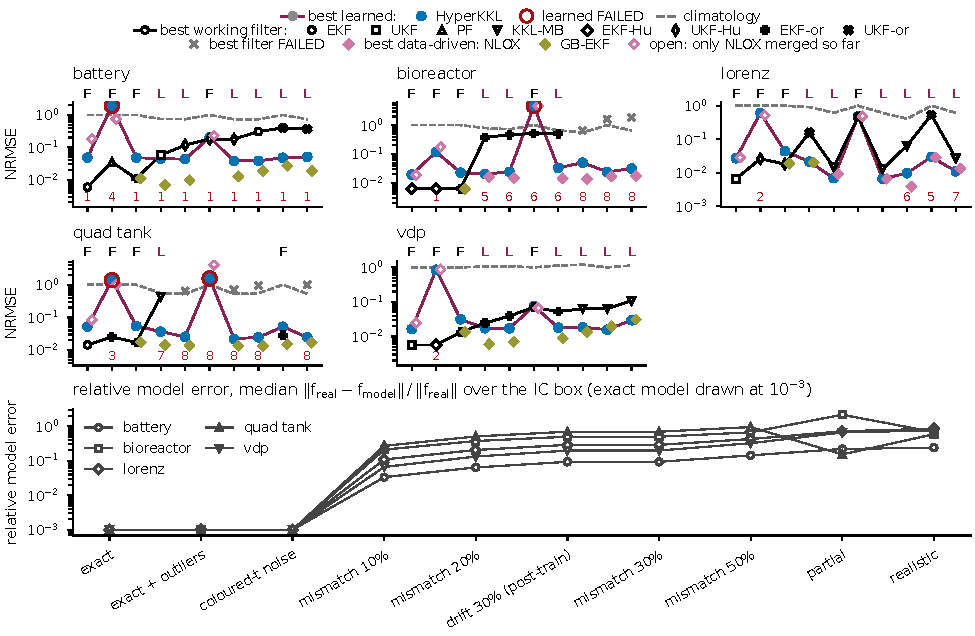
\includegraphics[width=0.85\textwidth]{fig3_c3_crossover_id.pdf}
\caption{As Figure~\ref{fig:c3}, in-distribution tier (\tier{id}). Climatology for \tier{id} is analytic for the nominal plant and a proxy for a perturbed plant (Appendix~\ref{app:protocol}).}
\label{fig:c3id}
\end{figure}

\begin{figure}[p]
\centering
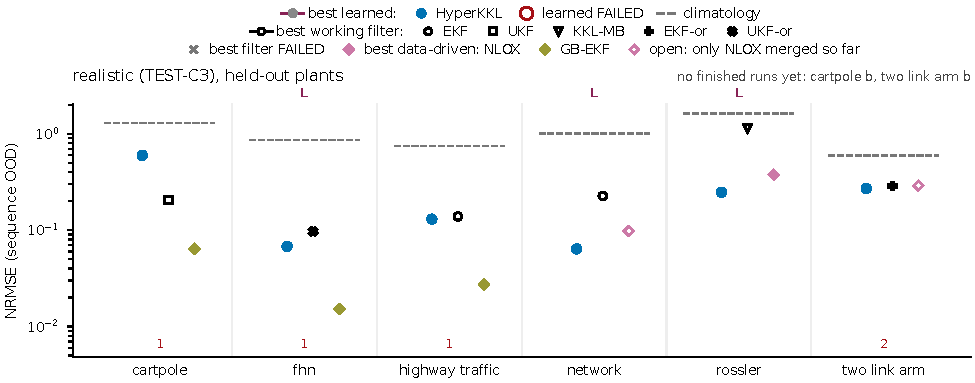
\includegraphics[width=0.85\textwidth]{fig3_c3_crossover_test.pdf}
\caption{As Figure~\ref{fig:c3} for the held-out plants under the realistic deployment (\node{TEST-C3}, frozen recipe, run once): \OutcomeTESTCThree\ at the time of generation (\JobsTESTCThree\ jobs finished); plants without finished runs are marked PENDING.}
\label{fig:c3test}
\end{figure}

\FloatBarrier
\subsection{C2: forgetting floor, memory probe and window sweeps}
\begin{figure}[tbp]
\centering
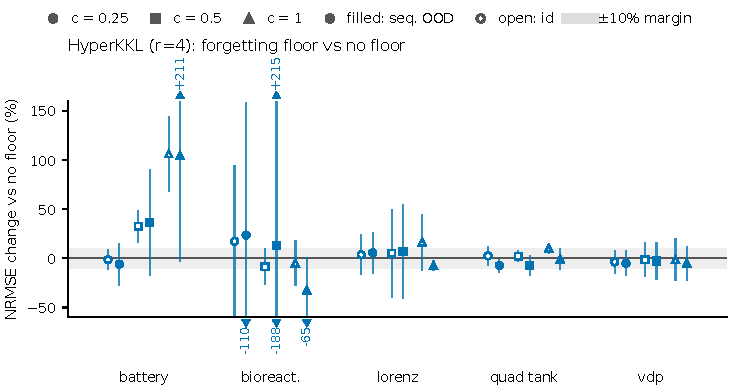
\includegraphics[width=\textwidth]{fig2a_c2_floor.pdf}
\caption{C2 forgetting-floor intervention: change in NRMSE when the SFM context is forced to forget at $\ge c\alpha$, relative to no floor (paired, 3 seeds, 95\% CI; grey band: $\pm10\%$ equivalence margin). The pre-registered rule at $c=0.5$ fails. }
\label{fig:c2floor}
\end{figure}

\begin{figure}[tbp]
\centering
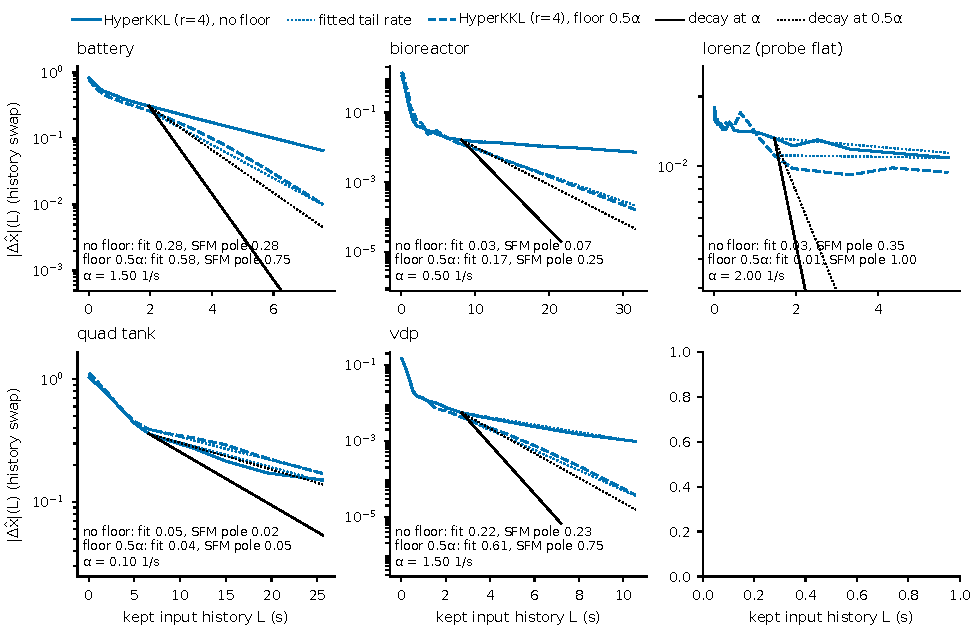
\includegraphics[width=\textwidth]{fig2b_c2_probe.pdf}
\caption{C2 memory probe (\tier{id}, 16 episodes, geometric mean over seeds): decoded change $|\Delta\hat x|$ when the last $L$ seconds of input are kept and everything older is swapped for another episode's input, with and without a $0.5\alpha$ forgetting floor. Black lines: decay at the design rate $\alpha$ (Lemma~\ref{lem:m2-tail}) and at $0.5\alpha$; coloured dotted lines: fitted tail rates. The \sys{lorenz} probe is flat.}
\label{fig:c2probe}
\end{figure}

\begin{figure}[tbp]
\centering
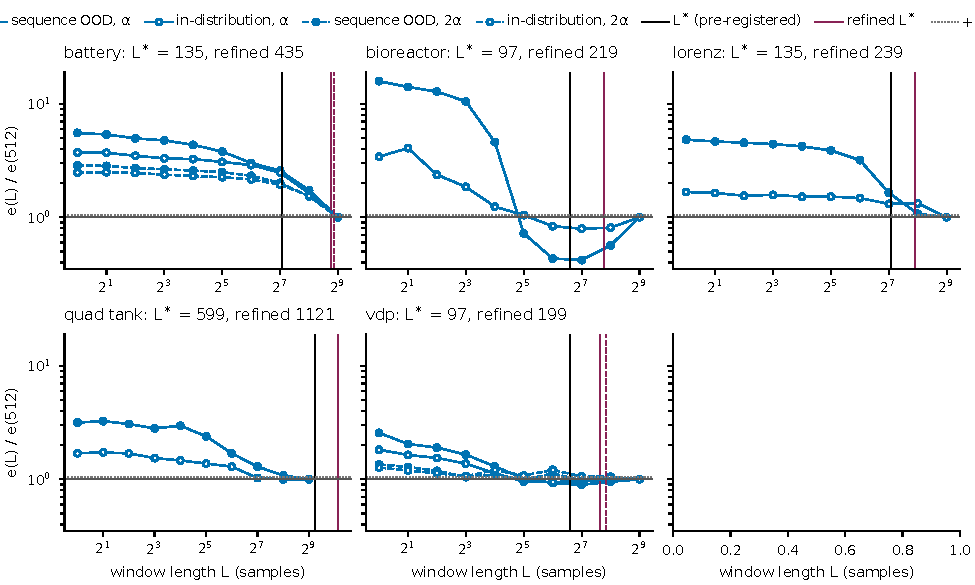
\includegraphics[width=\textwidth]{fig2c_c2_window.pdf}
\caption{C2 window sweeps (HyperKKL $r=4$ with a raw window encoder, mean over 3 seeds): $e(L)/e(512)$ against the window length in samples at the default bandwidth and, on three plants, at $2\alpha$. Black: pre-registered window $L^*=\ln(1/\eta)/\alpha$ ($\eta=0.05$); wine: refined $L^*=(\ln(1/\eta)+\ln\ell)/\alpha$ with the phase-1 proxy for $\ell$ (post hoc). Dotted: $+5\%$.}
\label{fig:c2window}
\end{figure}

\FloatBarrier
\subsection{Deployment scorecard}
\begin{figure}[p]
\centering
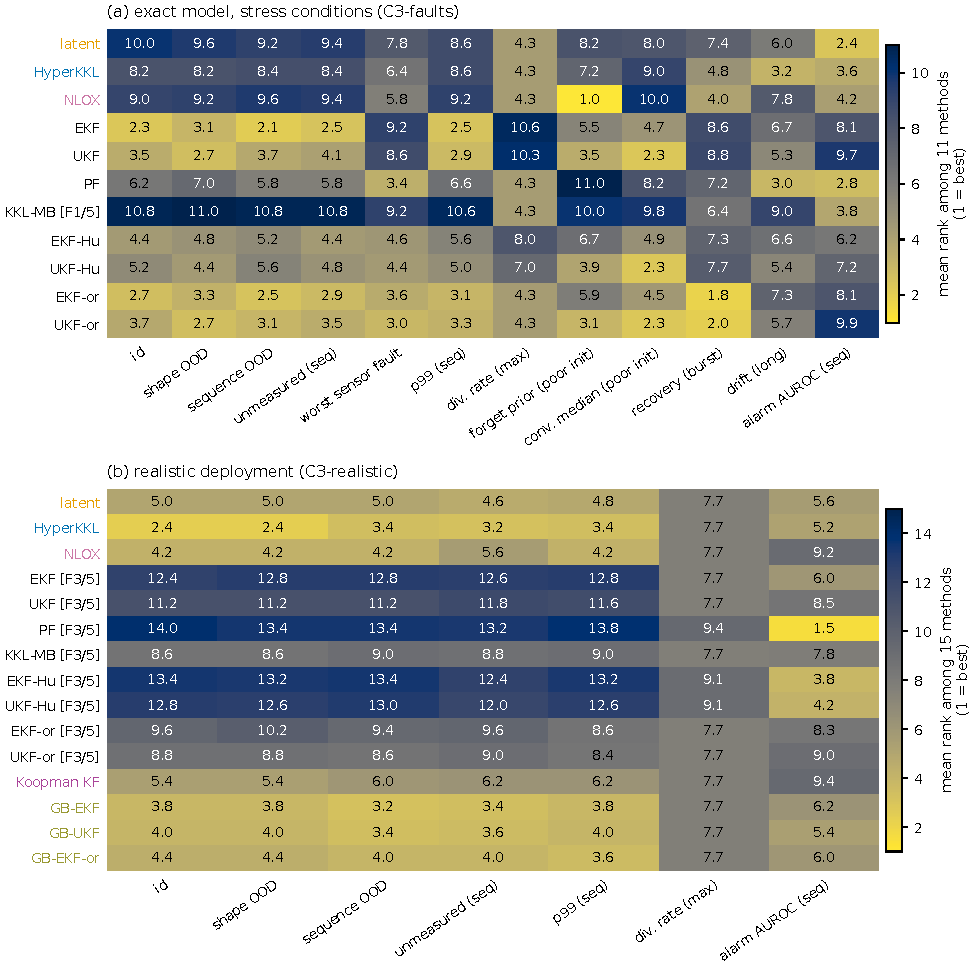
\includegraphics[width=0.95\textwidth]{fig4_scorecard.pdf}
\caption{Deployment scorecard as mean rank per column over the dev plants (1 = best). (a) exact model under the stress conditions of \node{C3-faults}; (b) realistic deployment (\node{C3-realistic}). [F$k$/6]: the method's \tier{sequence\_ood} NRMSE is above climatology on $k$ of six plants.}
\label{fig:scorecard}
\end{figure}
\inputonce{generated/tab3_scorecard_realistic}

\FloatBarrier
\subsection{Every decision rule}
\inputonce{generated/tab4_decisions}
